\subsection{Was sind Vektoren?}

Ein Vektor hat drei Eigenschaften:\\
\begin{itemize}
    \item Richtung
    \item Betrag/Länge
    \item Orientierung
\end{itemize}
Dadurch wird er grafisch als Pfeil dargestellt. Die Richtung wird durch die (Schräg-) Lage des Pfeils festgelegt.
Sein Betrag entspricht der Länge des Pfeils. Die Orientierung ergibt sich daraus, an welchem Ende des Pfeils die Spitze liegt.
Die Position eines Vektors spielt keine Rolle.

\hfill \break
Diese drei Pfeile stellen immer den gleichen Vektor dar, weil die Richtung, die Länge und die Orientierung bei allen gleich sind.

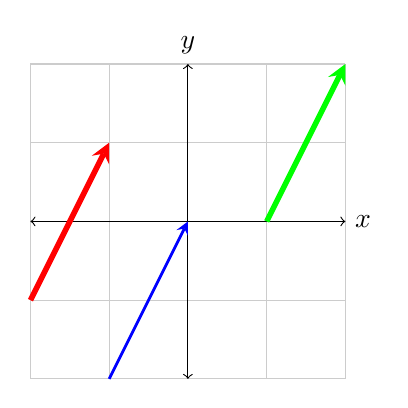
\begin{tikzpicture}
    \draw[thin,gray!40] (-2,-2) grid (2,2);
    \draw[<->] (-2,0)--(2,0) node[right]{$x$};
    \draw[<->] (0,-2)--(0,2) node[above]{$y$};
    \draw[line width=2pt,red,-stealth](-2,-1)--(-1,1) node[anchor=south west]{};
    \draw[line width=1pt,blue,-stealth](-1,-2)--(0,0) node[anchor=south west]{};
    \draw[line width=2pt,green,-stealth](1,0)--(2,2) node[anchor=south west]{};
\end{tikzpicture}

\break
Diese beiden Vektoren haben die gleiche Richtung und den gleichen Betrag.
Sie unterscheiden sich nur in ihrer Orientierung. Sie sind zueinander die Gegenvektoren.

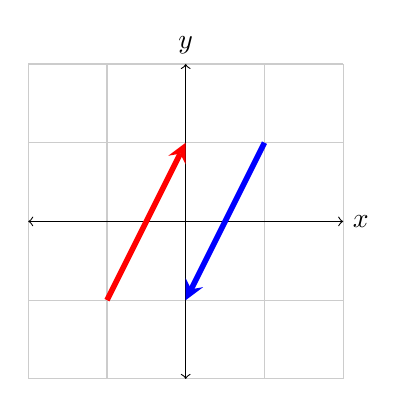
\begin{tikzpicture}
    \draw[thin,gray!40] (-2,-2) grid (2,2);
    \draw[<->] (-2,0)--(2,0) node[right]{$x$};
    \draw[<->] (0,-2)--(0,2) node[above]{$y$};
    \draw[line width=2pt,red,-stealth](-1,-1)--(0,1) node[anchor=south west]{};
    \draw[line width=2pt,blue,-stealth](1,1)--(0,-1) node[anchor=north east]{};
\end{tikzpicture}


\hfill \break
Für die Berechnung werden Vektoren ähnlich wie beim Steigungsdreieck von linearen Funktionen durch Komponenten entlang der Achsen dargestellt.

\hfill \break
Daher können Vektoren immer als Zahlenpaare dargestellt werden.
(Es gibt auch Vektoren im Raum, die mit 3 Komponenten dargestellt werden.)
Ob das Dreieck über oder unter dem Vektor gezeichnet wird, spielt keine Rolle.\\
$$\vec{a} = \binom{a_1}{a_2}$$